\documentclass[10pt, conference, compsocconf]{IEEEtran}

\usepackage{cite}
\ifCLASSINFOpdf
  \usepackage[pdftex]{graphicx}
  % declare the path(s) where your graphic files are
  \graphicspath{{../pdf/}{../jpeg/}}
  % and their extensions so you won't have to specify these with
  % every instance of \includegraphics
  \DeclareGraphicsExtensions{.pdf,.jpeg,.png}
\else
  % or other class option (dvipsone, dvipdf, if not using dvips). graphicx
  % will default to the driver specified in the system graphics.cfg if no
  % driver is specified.
  \usepackage[dvips]{graphicx}
  % declare the path(s) where your graphic files are
  \graphicspath{{../eps/}}
  % and their extensions so you won't have to specify these with
  % every instance of \includegraphics
  \DeclareGraphicsExtensions{.eps}
\fi

% *** FLOAT PACKAGES ***
%
\usepackage{fixltx2e}
% fixltx2e, the successor to the earlier fix2col.sty, was written by
% Frank Mittelbach and David Carlisle. This package corrects a few problems
% in the LaTeX2e kernel, the most notable of which is that in current
% LaTeX2e releases, the ordering of single and double column floats is not
% guaranteed to be preserved. Thus, an unpatched LaTeX2e can allow a
% single column figure to be placed prior to an earlier double column
% figure. The latest version and documentation can be found at:
% http://www.ctan.org/tex-archive/macros/latex/base/

\usepackage{url}
\usepackage[utf8]{inputenc}
\usepackage[T1]{fontenc}
%\usepackage[colorinlistoftodos,textsize=footnotesize,textwidth=1cm]{todonotes}
\usepackage[disable]{todonotes}
\usepackage{booktabs}
\usepackage{multirow}
\usepackage{array}
\usepackage[cmex10]{amsmath}
\usepackage[caption=false]{subfig}
\usepackage{rotating}
\usepackage{xcolor}
\usepackage{colortbl}
\usepackage[font=footnotesize]{caption}


\newcolumntype{v}[1]{>{\raggedright \hspace {0pt}}p{#1}}
\def\IEEEbibitemsep{4pt plus 1.6pt}

% correct bad hyphenation here
\hyphenation{op-tical net-works semi-conduc-tor}

% Avoid orphans and widows (thx IEEE help!)
          \clubpenalty = 10000
          \widowpenalty = 10000
          \displaywidowpenalty = 10000

% Balance columns on last page (thx IEEE help!)
          \usepackage{balance}

\begin{document}



% For peer review papers, you can put extra information on the cover
% page as needed:
% \ifCLASSOPTIONpeerreview
% \begin{center} \bfseries EDICS Category: 3-BBND \end{center}
% \fi
%
% For peerreview papers, this IEEEtran command inserts a page break and
% creates the second title. It will be ignored for other modes.
\IEEEpeerreviewmaketitle

% !TEX root = knauss-vissuelizer.tex
\pdfinfo{/Author (Eric Knauss, Daniela Damian) 
/Title (V:issue:lizer: Explore Online Communication) 
/Subject () 
/Keywords (Requirements clarification patterns; distributed requirements engineering; communication of requirements)}

\title{V:issue:lizer\\Explore Online Communication and  Requirements Clarification over Time}


\author{\IEEEauthorblockN{Eric Knauss, Daniela Damian}
\IEEEauthorblockA{SEGAL, University of Victoria, Victoria B.C., Canada\\
knauss@computer.org, danielad@cs.uvic.ca
}}

\maketitle


\begin{abstract}
This demo introduces \viss\ as a tool for exploring online communication and analysing clarification of requirements over time.
\viss\ enables managers to identify hotspots in current development activities, to analyze communication problems, and to identify developers that are knowledgeable about domain or project related issues by offering powerful visualizations.
Our preliminary evaluation shows that \viss\ offers managers valuable information for their decision making.
\end{abstract}

\begin{IEEEkeywords}
requirements clarification patterns; distributed requirements engineering; communication of requirements
\end{IEEEkeywords}

% !TEX root = knauss-vissuelizer.tex
\section{Introduction}

Large software projects are often affected by the need to collaborate across geographically distributed sites and to depend upon online communication to perform requirements related activities. 
More and more teams employ agile approaches that aim at discovering requirements iteratively and rely on frequent communication instead of requirements documentation. 
In such approaches, requirements are defined in the form of user stories, and ongoing discussions around these user stories serve as the main mechanism to clarify the meaning of requirements and to coordinate their implementation \cite{Cao2008}. 
Recording such discussions and decisions in online project repositories is an emerging best practice, not only in large and distributed projects \cite{Aranda2007}.
IBM\textsuperscript{\textregistered}'s Rational Team Concert\textsuperscript{\textregistered} project, with a large distributed team, is an example in which management mandates the recording of all decisions in the project repository for future use in the project\cite{Frost2007}. 
Consequently, online project repositories contain a wealth of requirements-related communication.

In these kinds of environments, however, the expected evolution of a requirement from an initial idea, through clarification, to design and full implementation, often stagnates. 
%Process-related issues, inadequate tool support or inadequate communication [refs) are common reasons for such problems. 
E.g. stakeholders continue to \emph{clarify} the requirement because it is ambiguous, incomplete, or has frequent changes. 
As a result, its implementation can be delayed or sometimes never get started. 
%Bikeshedding, also known as the Parkinson's law of triviality\cite{Parkinson1958} is another common situation in which developers give disproportionate weight and time to solving trivial issues and delay development. 
%An example from the RTC project (jazz.net) is the ongoing discussion of a large number of developers over the  text required in a UI element, and which blocked the development of this user story. 
%Late in the project a manager intervenes and makes a decision "we go with [...] for this iteration", after which development of the story is completed. 
%Although with a happy ending, many situations like this go unnoticed by managers. 
Current requirements management tools offer little support for identifying requirements with progression problems, thereby lowering the project manager's  ability to intervene in a timely manner.

%\begin{figure}[h]
%\begin{center}
%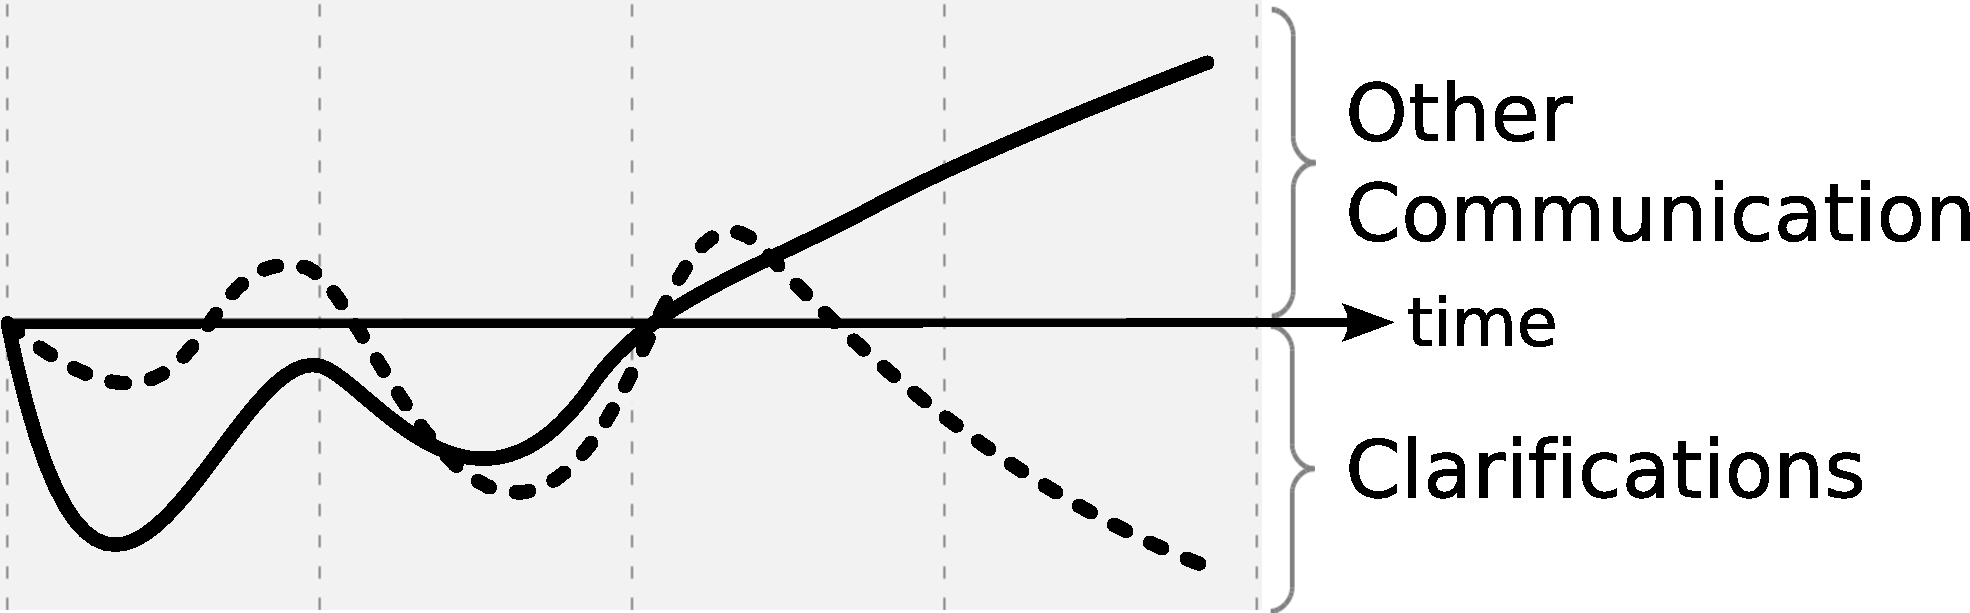
\includegraphics[width=0.7\columnwidth]{img/basic-pattern}
%\caption{Two different trajectories of reqts. communication}
%Predominance of clarifications in requirements-related communication may be problematic }
%\label{fig:basic-pattern}
%\end{center}
%\end{figure}

%Studying recorded online communication fills this gap by offering the potential to reveal patterns of communication that correlate to problematic situations around requirements development. 
In this demo we present a novel tool for analyzing online communication and differentiating between healthy and problematic patterns of communication associated with an individual requirement. 
Our \viss\ tool helps managers to analyze the content of communication among stakeholders involved in the discussion of a particular requirement, identify specific instances of \emph{clarifying} communication, and examine the trajectory of clarifications (i.e. amount of communication and progression) throughout the lifetime of a requirement. 
%Figure \ref{fig:basic-pattern} shows two distinct and quite different possible trajectories of \emph{clarifying} communication in the lifetime of a requirement. 
%While one would expect clarification to diminish as development of a requirement nears the end (solid line trajectory), its predominance throughout the requirement's life may be indicative of problematic requirements (dashed line trajectory). 
%The method proposed in this paper aims to identify these patterns automatically so that managers or involved stakeholders can be made aware of requirements that should be closely investigated.
In addition, \viss\ can visualize social networks that allow to assess the constellation of communication actors and to identify experts for given topics.

%Figure \ref{fig:basic-pattern} depicts the characteristics of clarification communication related to a requirement (here: a story in Jazz).


%The contribution of this paper is the method for the detection and classification of clarification communication patterns, as well as a set of six communication patterns that we identified by applying our method in a large industrial project. 
%The remainder of the paper is structured as follows: Section \ref{sec:relatedwork} surveys related work in the study of communication in requirements engineering (RE), as well as related to information retrieval and automated classification techniques in RE. 
%Section \ref{sec:approach} introduces our research approach in studying requirements communication and the set of our techniques for the detection and classification of clarification  patterns. 
%We then describe the details of the industrial case study in which we applied our techniques in Sections \ref{sec:classification}, \ref{sec:visualization-and-patterns}, \ref{sec:recommendations} and \ref{sec:discussion}, and 
%give a detailed description of the three primary phases of our method: \emph{classification of requirements discussions}, \emph{clarification patterns development} and  \emph{pattern classification}.  
% conclude with future research steps in Section \ref{sec:conclusion}.

%\subsection{Background}
%The Jazz team uses Jazz as collaboration platform. It is the goal of the team to capture the entire communication in comments to \emph{workitems}. One of the workitem types, the \emph{story} contains requirements. Jazz follows an agile development approach, i.e. stories are refined during the project. This includes the decomposition in sub-workitems, most often of the workitem-type \emph{task}. 

%For a given requirement, the graph shows how the amount of clarification changes over time. 
%The example in the figure shows  a reoccurring characteristic that follows one of our six clarification communication patterns: the \emph{perfect clarification} pattern.


%Online communication to perform requirements related activities, such as elicitation, negotiation or development of requirements, is a critical part of large modern software projects. 
%Stakeholders in today's large software projects, most often at geographically distributed sites, largely rely on online communication in their collaboration. 
%Whether they follow an iterative discovery of requirements as in agile projects \cite{Cao2008}, or the time zone differences between stakeholders are too great to allow for frequent synchronous interaction (ref)2, or follow processes that mandate the recording of requirements communication online (ref3), these stakeholders perform various Requirements Engineering related activities through online communication. 

We conducted a preliminary evaluation in two ways. Firstly, we evaluated \viss's ability to correctly identify communication instances concerned with clarification and it's ability to derive meaningful visualizations of the clarification trajectory \cite{Knauss2012f}. 
Secondly, we confronted software managers with \viss's visualizations and asked them, whether the visualization was useful, if it did offer information they would have missed otherwise, and what actions they would perform based on the feedback, if any. 

\begin{figure*}
\centering
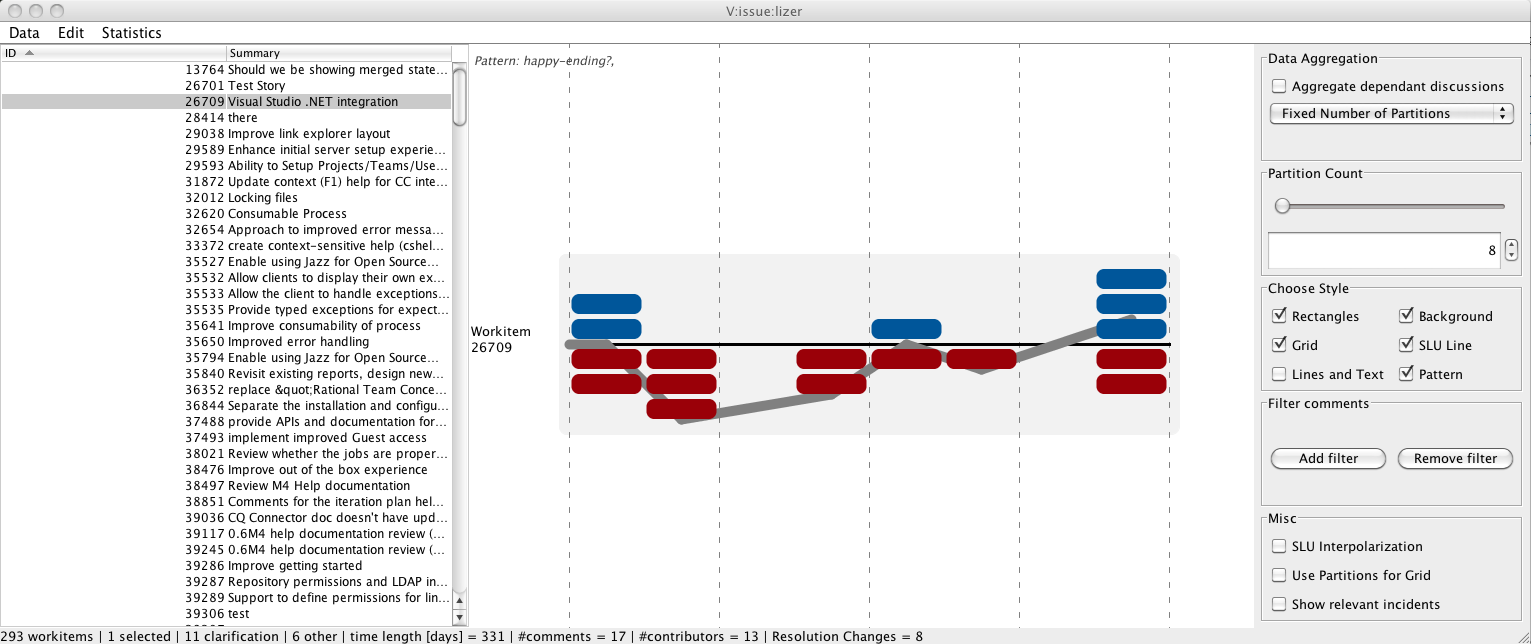
\includegraphics[width=0.8\textwidth]{img/vissuelizer-screenshot}
\caption{Screenshot: the main window of the \viss\ shows a list of issues (e.g. user stories) and their clarification trajectories.}
\label{fig:screenshot}
\end{figure*}
%\input{relatedwork}
%\input{approach}
%\input{classification}
%\input{visualization}
%\input{recommendations}
%\input{discussion}
%% !TEX root = knauss-vissuelizer.tex
\section{Conclusion and Future Work}
\todo[inline]{Dana, please review conclusion}
With \viss\ we introduced a visualization tool to analyze requirements clarification in online communication over time.
Especially agile and distributed projects demand such analysis: agile projects often only sketch requirements in sufficient detail to plan the next iteration and leave the details to be clarified during the development; distributed projects often depend on online communication and challenge their project managers' ability to assess the shared understanding in the team. 
Our preliminary evaluation has shown that our visualizations allow managers to identify hotspots, e.g. user stories that are not clear to the team. 
Furthermore, \viss\ supports managers in investigating the cause of those hotspots and in identifying suitable actions to disarm problematic or risky situations where the team has insufficient understanding of requirements.
 
In future work, we will evaluate how practitioners use our tool in their daily work. 
This will help us to gain further insight on how managers can use information about requirements clarification over time and to quantify the benefits that tools like the \viss\ can offer.

Such further evaluation should also relate features of online communication (i.e. network centrality, late clarification, no clarification) with typical problems of requirements related discussions, such as feature creep \cite{Jones1996} or symmetry of ignorance \cite{Fischer2000}.

\section*{Acknowledgements}
\todo[inline]{There is a number of people we should acknowledge.}
%\vspace{-1cm}
\balance

\listoftodos

\bibliographystyle{IEEEtran}
\bibliography{IEEEabrv,bibliography}
\end{document}
